\documentclass[11pt, english, fleqn, DIV=15, headinclude, BCOR=1.5cm]{scrartcl}

\usepackage[
    bibatend,
    %color,
]{../header}

\usepackage{tikz}
\usepackage{pdflscape}

\usepackage[tikz]{mdframed}
\newmdtheoremenv[%
    backgroundcolor=black!5,
    innertopmargin=\topskip,
    splittopskip=\topskip,
]{theorem}{Theorem}[section]

\hypersetup{
    pdftitle=
}

\newcounter{totalpoints}
\newcommand\punkte[1]{#1\addtocounter{totalpoints}{#1}}

\newcounter{problemset}
\setcounter{problemset}{9}

\subject{physics606 -- Advanced Quantum Theory}
\ihead{physics606 -- Problem Set \arabic{problemset}}

\title{Problem Set \arabic{problemset}}

\publishers{Group 2 -- Dilege Gülmez}
\ofoot{Group 2 -- Dilege Gülmez}

\newmdenv[%
    backgroundcolor=black!0,
    frametitlebackgroundcolor=black!0,
    roundcorner=5pt,
    skipabove=\topskip,
    innertopmargin=\topskip,
    splittopskip=\topskip,
    frametitle={Problem statement},
    frametitlerule=true,
    nobreak=true,
]{problem}

\newmdenv[%
    backgroundcolor=white,
    frametitlebackgroundcolor=black!0,
    roundcorner=5pt,
    skipabove=\topskip,
    innertopmargin=\topskip,
    innerbottommargin=8cm,
    splittopskip=\topskip,
    frametitle={Side question},
    frametitlerule=true,
]{question}

\newcommand\an{^\text{angular}}
\newcommand\ra{^\text{radial}}


\author{
    Martin Ueding \\ \small{\href{mailto:mu@martin-ueding.de}{mu@martin-ueding.de}}
    \and
    Lino Lemmer \\ \small{\href{mailto:l2@uni-bonn.de}{l2@uni-bonn.de}}
}
\ifoot{Martin Ueding, Lino Lemmer}

\ohead{\rightmark}

\begin{document}

\maketitle

\vspace{3ex}

\begin{center}
    \begin{tabular}{rrr}
        problem number & achieved points & possible points \\
        \midrule
        1 & & \punkte{15} \\
        2 & & \punkte{15} \\
        \midrule
        total & & \arabic{totalpoints}
    \end{tabular}
\end{center}

\section{Expansion of a plane wave}

\subsection{Spherical Bessel functions}

We start with the definition.
\begin{align*}
    j_l(x)
    &= - x^l \sbr{\frac 1x \od{}x}^l \frac{\sin(x)}{x} \\
    \intertext{%
        Now we insert the series expansion of the sinc function.
    }
    &= - x^l \sbr{\frac 1x \od{}x}^l \sum_{n=0}^\infty \frac{[-1]^n}{[2n+1]!}
    x^{2n} \\
    \intertext{%
        Commuting terms.
    }
    &= - \sum_{n=0}^\infty \frac{[-1]^n}{[2n+1]!} x^l \sbr{\frac 1x \od{}x}^l
    x^{2n} \\
    \intertext{%
        The big square bracket will decrease the power of $x^{2n}$ by $2l$ in
        total. Only terms with $n \geq l$ will contribute. We will omit higher
        terms. This leaves only one interesting term, we can drop the sum and
        set $n = l$.
    }
    &= - \frac{[-1]^l}{[2l+1]!} x^l \sbr{\frac 1x \od{}x}^l x^{2l} + \mathcal O(x^{l + 2}) \\
    \intertext{%
        The factors that we get by differentiating is every second of $2l,
        2l-2, 2l-4, \ldots =: [2l]!!$.
    }
    &= - \frac{[-1]^l [2l]!!}{[2l+1]!} x^l + \mathcal O(x^{l + 2}) \\
    \intertext{%
        Realizing that
        \[
            [2l]!!
            = [2l][2l-2][2l-4]\ldots
            = 2 l 2 [l-1] 2 [l-2] \ldots
            = 2^l l!
        \]
        gives
    }
    &= [-1]^{l+1} \frac{2^l l!}{[2l+1]!} x^l + \mathcal O(x^{l + 2})
\end{align*}
This result differers from the result on the problem set by the $l$ dependent
sign.

\subsection{Expression of $x^l$}

We only look at the highest term in the Legendre polynomial:
\[
    P_l(x)
    = \frac{1}{2^l l!} \od{^l}{x^l} \sbr{x^{2l} + \ldots}
    = \frac{1}{2^l l!} \frac{[2l]!}{l!} x^{l} + \ldots
\]
The other terms contain lesser powers of $x$ than $x^l$. Then this can be
inverted to
\[
    x^l = \frac{2^l [l!]^2}{[2l]!} P_l(x) + \ldots.
\]

\subsection{Use of orthogonality}

We define $\xi := \cos(\theta)$ for this subsection. It is slightly confusing
that $k$ is used as the wave number and an index, we use $m$ instead.

Start with expansion of plane wave.
\begin{align*}
    \exp(\iup k x \xi) &= \sum_{l = 0}^\infty A_l j_l(kx) P_l(\xi) \\
    \intertext{%
        $L^2$ project this onto $P_m(\xi)$.
    }
    \int_{-1}^1 \dif \xi \, P_m(\xi) \exp(\iup k x \xi) &= \sum_{l = 0}^\infty A_l
    j_l(kx) \int_{-1}^1 \dif \xi \, P_m(\xi) P_l(\xi) \\
    \intertext{%
        Use orthogonality.
    }
    \int_{-1}^1 \dif \xi \, P_m(\xi) \exp(\iup k x \xi) &= \sum_{l = 0}^\infty A_l
    j_l(kx) \frac{2}{2l+1} \delta_{lm} \\
    \intertext{%
        Execute $\delta$.
    }
    \int_{-1}^1 \dif \xi \, P_m(\xi) \exp(\iup k x \xi) &= A_m
    j_m(kx) \frac{2}{2k+1} \\
    \intertext{%
        Move fraction to other side.
    }
    \frac{2m+1}{2} \int_{-1}^1 \dif \xi \, P_m(\xi) \exp(\iup k x \xi) &= A_m
    j_m(kx)
\end{align*}
This is not the result on the problem set, since the integration measure
$\dif\cos(\theta) = \dif\xi$ is missing there.

\subsection{Extraction of $A_l$}

We start with the expression we just derived.
\begin{align*}
    A_l j_l(kx)
    &= \frac{2l+1}{2} \int_{-1}^1 \dif \xi \, P_l(\xi) \exp(\iup k x \xi) \\
    \intertext{%
        We express $j_l$ through its approximation around $kx = 0$ and express
        $P_l$ in terms of $x$.
    }
    A_m [kx]^l \frac{2^l l!}{[2l+1]!}
    &= \frac{2l+1}{2} \int_{-1}^1 \dif \xi \, \frac{[2l]!}{2^l[l!]^2} \xi^l \exp(\iup k x \xi) \\
    \intertext{%
        Next we insert the \emph{definition} of the exponential.
    }
    A_m [kx]^l \frac{2^l l!}{[2l+1]!}
    &= \frac{2l+1}{2} \int_{-1}^1 \dif \xi \, \frac{[2l]!}{2^l[l!]^2} \xi^l
    \sbr{1 + \iup k x \xi + \mathcal O(\xi^2)} \\
    \intertext{%
        We move the Landau $\mathcal O$ out of the integral.
    }
    A_m [kx]^l \frac{2^l l!}{[2l+1]!}
    &= \frac{2l+1}{2} \int_{-1}^1 \dif \xi \, \frac{[2l]!}{2^l[l!]^2} \xi^l
    [1 + \iup k x \xi] + \mathcal O(\xi^{l+2}) \\
    \intertext{%
        Move the factors to the right hand side.
    }
    A_m &= \frac{[2l+1]!}{2^l l!} \frac{2l+1}{2} \frac{1}{[kx]^l}
    \frac{[2l]!}{2^l[l!]^2} \int_{-1}^1 \dif \xi \, \xi^l [1 + \iup k x \xi] +
    \mathcal O(\xi^{l+2}) \\
    \intertext{%
        Simplify.
    }
    A_m &= [2l+1]! [2l+1] \frac{[2l]!}{2^{2l+1} [l!]^3} \frac{1}{[kx]^l}
    \int_{-1}^1 \dif \xi \, \xi^l [1 + \iup k x \xi] + \mathcal O(\xi^{l+2}) \\
    A_m &= [2l+1]^2 \frac{\sbr{[2l]!}^2}{2^{2l+1} [l!]^3} \frac{1}{[kx]^l}
    \int_{-1}^1 \dif \xi \, \xi^l [1 + \iup k x \xi] + \mathcal O(\xi^{l+2})
\end{align*}
One of the integrals will give zero, the other will contribute something that
only depends on $kx$.

\section{Scattering on a dipole}

\subsection{Scattering amplitude}

Figure~\ref{fig:sketch} shows the two scattering centers as well as the
incoming and outgoing wave vectors. The $\Deltaup s$ and $\Deltaup s'$ are the
path differences for the two vectors. The incident waves are in phase and have
the same wave vector $\vec k$. The incoming waves, represented by two wave
vectors, scatter at the respective positions. At the point where they scatter,
they have a phase shift due to the path difference. The path difference
$\Deltaup s$ is the projection of $\vec d$ onto the direction of $\vec k$,
namely
\[
    \Deltaup s = \vec d \frac{\vec k}{k}.
\]
The phase shift is this distance times the wave number, so the phase difference
is given by the scalar product
\[
    \Deltaup \phi = \vec d \vec k.
\]

\begin{figure}[htbp]
    \centering
    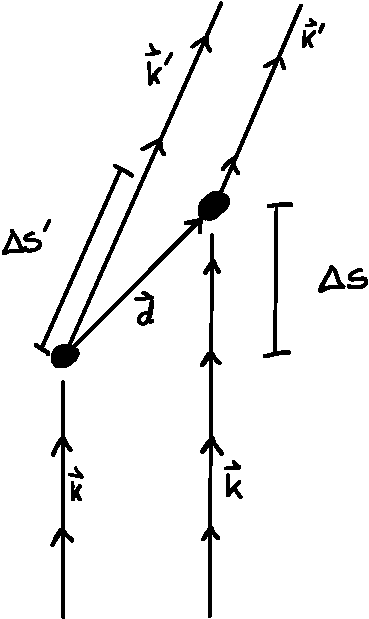
\includegraphics{Drawing-0001.pdf}
    \caption{%
        Path difference for the two scattered waves.
    }
    \label{fig:sketch}
\end{figure}

A similar thing happens for the scattered waves, they also have a path
difference. In the case where $\vec k$ and $\vec d$, as well as $\vec k'$ and
$\vec d$ point into the same direction (such that $\vec k \vec d > 0 \land \vec
k' \vec d > 0$), like in the picture, the path difference has a negative sign
now. For the incoming wave, the right wave had an additional path, now it is
the left wave with the additional path. We count this negatively then. The
phase shift here is
\[
    \Deltaup \phi' = - \vec d \vec k'.
\]

The total phase shift therefore is
\[
    \vec d [\vec k - \vec k']
    =
    \vec d \vec q.
\]
Equation~(10) on the problem set gives the monopole scattering amplitude. It
depends on the charge of the particles. Since the second particle has opposite
charge, we will get the negative of the amplitude. Adding both amplitudes with
the phase shift gives us the desired
\[
    f_{\vec k}^\text{dipole}
    = \sbr{1 - \exp(- \iup \vec q \vec d)} f_{\vec k}^\text{monopole}.
\]

\subsection{Case of aligned dipole}

We have
\[
    \vec d =
    \begin{pmatrix}
        0 \\ 0 \\ d
    \end{pmatrix}.
\]
Then
\[
    \vec q \vec d = [1 - \cos(\theta)] kd.
\]
This part is independent of $\phi$. Then we need $f^\text{monopole}_{\vec k}$:
\begin{align*}
    f^\text{monopole}_{\vec k}
    &= - \frac{2M}\hbar \frac{Z_1 Z_2 e^2}{4 \piup \varepsilon_0} \frac{1}{q^2}
    \\
    \intertext{%
        We insert $\vec q$.
    }
    &= - \frac{2M}\hbar \frac{Z_1 Z_2 e^2}{4 \piup \varepsilon_0} \frac{1}{k^2}
    \frac{1}{\sin(\theta^2) \sin(\phi)^2 + \sin(\theta)^2 \cos(\phi)^2 +
    [1-\cos(\theta)]^2}
    \intertext{%
        We use trigonometric identities to simplify.
    }
    &= - \frac{2M}\hbar \frac{Z_1 Z_2 e^2}{4 \piup \varepsilon_0} \frac{1}{k^2}
    \frac{1}{\sin(\theta^2) + \cos(\theta)^2 - 2 \cos(\theta) + 1} \\
    \intertext{%
        This can be simplified further.
    }
    &= - \frac{2M}\hbar \frac{Z_1 Z_2 e^2}{4 \piup \varepsilon_0} \frac{1}{k^2}
    \frac{1}{2 - 2 \cos(\theta)} \\
    \intertext{%
        For convenience, we introduce $\xi := 1 - \cos(\theta)$.
    }
    &= - \frac{2M}\hbar \frac{Z_1 Z_2 e^2}{4 \piup \varepsilon_0} \frac{1}{k^2}
    \frac{1}{2\xi} \\
    \intertext{%
        For even more convenience, we introduce $A$ to carry all the constant
        factors.
    }
    &= \frac{A}{k^2 \xi}
\end{align*}

The whole scattering amplitude then is
\begin{align*}
    f_{\vec k}^\text{dipole}
    &= \frac{A}{k^2} \frac{1 - \exp(- \iup \xi k d)}{\xi}.
    \intertext{%
        We write down the leading terms of the exponential function.
    }
    f_{\vec k}^\text{dipole}
    &= \frac{A}{k^2} \frac{\iup \xi k d + \mathcal O(\xi^2)}{\xi} \\
    \intertext{%
        We cancel $\xi$.
    }
    &= \frac{A}{k^2} \iup k d + \mathcal O(\xi)
\end{align*}
This is now well behaved in the limit $\theta \to 0$ implying $\xi \to 0$. It
will be a finite nonzero value.

\end{document}

% vim: spell spelllang=en tw=79
